\documentclass[c,8pt,xcolor...,x11names]{beamer}
\usepackage{icclslides}
\usepackage[latin1]{inputenc}
\usepackage[british]{babel}
\usepackage{amssymb}
\usepackage{latexsym}
\usepackage{rotate}
\usepackage{tikz}
\usepackage{verbatim}
\usepackage{colortbl}
\usepackage{booktabs}
\usepackage{ulem}
% \usepackage{arydshln}
\usepackage{pdfpages}
\usepackage{graphicx} 
\usepackage{tikz}
\usepackage{makecell}
\usepackage{tabularx}
\usepackage{makecell}
\usepackage{comment}
\newcolumntype{C}{>{${}}c<{{}$}}
\newcolumntype{d}[1]{D{,}{,}{#1}}
\usepackage{listings}

\lstdefinestyle{SC}{
	language=erlang,
	xleftmargin=.2\textwidth,
	xrightmargin=.2\textwidth
}
\lstset{ 
	basicstyle=\scriptsize,
	showstringspaces=false,
	showspaces=false,
	commentstyle=\color{blue},
	keywordstyle=\bfseries\color{purple},
	captionpos=b,
	frame=lines
}

%\usepackage{natbib}


\usetikzlibrary{positioning}
\newcommand\tab[1][1cm]{\hspace*{#1}}
\tikzstyle{ele} = [circle, text centered, minimum width=1em, minimum height=3ex]

%% Uncomment to activate navigation symbols in the lower right of the pages:
\setbeamertemplate{navigation symbols}{}

\renewcommand{\Myauthor}{Aneta Koleva}
\renewcommand{\Mytitle}{On Commonsense Domains within  the Winograd Schema Challenge}
\usepackage{showexpl} 

\lstloadlanguages{[LaTeX]Tex} 
\lstset{% 
     basicstyle=\ttfamily\small, 
     commentstyle=\itshape\ttfamily\small, 
     showspaces=false, 
     showstringspaces=false, 
     breaklines=true, 
     breakautoindent=true, 
     captionpos=t 
} 

\begin{document} 
\begin{frame}
\customtitle
\begin{list2}
\item Winograd Schema Challenge
\item Previous Approaches
\item Knowledge Types Identification and Reasoning
\item Categorization of Winograd Schemas
\item Conclusion
\end{list2}
\end{frame}


\section{Motivation} 


\begin{frame}
  \frametitle{Motivation}
	\onslide<1->\begin{itemize} 	
	\item Winograd Schema Challenge (Levesque et al., 2012)
	\begin{itemize}
		\normalsize
		\item[S:] The trophy does not fit into the brown suitcase\\ because \alert{it} is too \alert{[small/large]}.
		\item[Q:] What is too [small/large]?
		\item[A:] The suitcase/the trophy.
	\end{itemize}	
	
\end{itemize}
\onslide<2->		\centering
%\documentclass{article}
%\usepackage{tikz}
%\begin{document}
\begin{comment}
	content...

	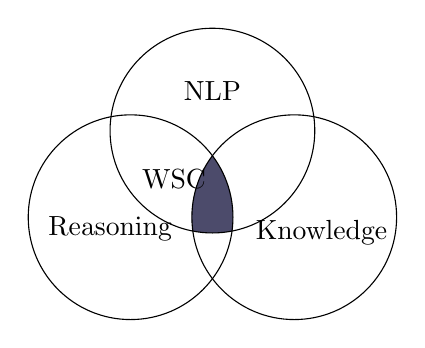
\begin{tikzpicture}
	\definecolor{Psy}{HTML}{4C4B6B}
	 \begin{scope}%[blend group=soft light]
	 
	 \def\firstcircle{( 90:0.5) circle (1.3cm)}
	 \def\secondcircle{(210:1.2) circle (1.3cm)}
	 \def\thirdcircle{(330:1.2) circle (1.3cm)}
	    \fill[white]  \firstcircle;
		 \fill[white] \secondcircle;
		 \fill[white] \thirdcircle;
		 
			 
		  \begin{scope}
		\clip \firstcircle;
		\clip \secondcircle;
		\fill[Psy] \thirdcircle;
		\end{scope}
			 
		 \draw \firstcircle;
		 \draw \secondcircle;
		 \draw \thirdcircle;
		 
		 \node at ( 90:1)    {NLP};
		 \node at (210:1.5)    {Reasoning};
		 \node at (330:1.6)    {Knowledge};
		 \node at (193:0.5) {WSC};
	\end{scope}	 
	\end{tikzpicture}
%
\end{comment}

\begin{figure}[width]
	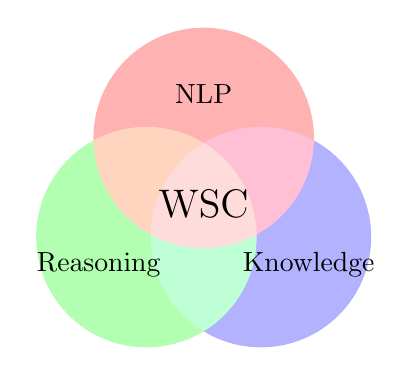
\begin{tikzpicture}[scale = 0.7]
	\begin{scope}[blend group = soft light]
	\fill[red!30!white]   ( 90:1.2) circle (2);
	\fill[green!30!white] (210:1.2) circle (2);
	\fill[blue!30!white]  (330:1.2) circle (2);
	\end{scope}
	\node at ( 90:2)    {NLP};
	\node at ( 210:2.2)   {Reasoning};
	\node at ( 330:2.2)   {{Knowledge}};
	\node [font=\Large] {WSC};
	\end{tikzpicture}
\end{figure}

%\end{document}%
\end{frame}

\begin{comment}
	content...

\begin{frame}
\vfill
\begin{LARGE}
\hfill Structure of a {\sc Beamer} Document \hfill 
\end{LARGE}
\vfill
\end{frame}
\end{comment}

\subsection{Winograd Schema Challenge}

\begin{frame}
\frametitle{Winograd Schema Challenge}
\onslide<1->	\begin{itemize}
	\small{
	\item[S:] The trophy does not fit into the brown suitcase\\ because \alert{it} is too \alert{[small/large]}.
	\item[Q:] What is too [small/large]?
	\item[A:] The suitcase/the trophy. }
\end{itemize} 
\onslide<2->\begin{itemize}
	\item Winograd Schema: 
	\begin{center}
	\begin{tabular}{ l | c }
		Sentence containing two nouns &  \alert{trophy}, \alert{suitcase} \\
		\hline 
		One ambiguous pronoun & \alert{it} \\  
		\hline
		A special word & \alert{small}/\alert{ large}\\
		\hline
		Question about the referent of the pronoun & What is too [\alert{small}/\alert{large}]\\
		\hline
		Two possible answers & \alert{The suitcase} /\alert{the trophy}\\
	\end{tabular}
	\end{center}


%	\begin{itemize}
%		\normalsize
%		\item Sentence containing two nouns, \\one ambiguous \alert{pronoun} and a special word
%		\item Question asking about the referent of the pronoun
%		\item Two possible answers corresponding to\\ the noun phrases in the sentence
%	\end{itemize}
	\onslide<3->	 \item Characteristics:
	\onslide<3->	  \begin{itemize}
		\normalsize
		\item Easy to answer for an adult English speaker
		\item Always contains \alert{special word}
		\item Google proof
	\end{itemize}
\end{itemize}
\end{frame}

\subsection{Competition}

\begin{frame}
\frametitle{Competition}
	\begin{itemize}
	\normalsize
	\item Competition in 2016 at IJCAI-16
	\begin{itemize}
		\normalsize
		\item Two time-constraint rounds - 210 min. each
		\begin{itemize}
			\normalsize
			\item Pronoun Disambiguation Problems (PDPs) - 60
			\item Parts of Winograd Schemas - 150
		\end{itemize}
		\item Four competitors
		\item Best result: 58\% correctly resolved PDPs
		\item There was no second round
		
	\end{itemize}
	
	\item Current \alert{state-of-the-art} (Radford et al., 2019) achieves \\ 70.7\% accuracy on the WSs dataset
\end{itemize}
\end{frame}

\section{Previous Approaches}

\begin{frame}
\frametitle{Previous Approaches}
\onslide<1->\begin{itemize}
	\item Machine learning and deep learning techniques
	\item Knowledge-based system with reasoning procedures
\end{itemize}

\onslide<2->
\setlength{\tabcolsep}{2pt}
\renewcommand{\arraystretch}{2}
%\setlength{\extrarowheight}{3pt}

{\footnotesize
	
\hspace*{-0.6cm} 	\begin{tabularx}{\textwidth}{ l|c c c l}
		
\onslide<2->{\makecell[c]{\textbf{Technique}}  &{\makecell[c]{\textbf{PDPs}\\ Size - Correct}} &{\makecell[c]{\textbf{WSC}\\Size - Correct}} &{\makecell[c]{{\textbf{WSC*}}\\Size - Correct}} &\makecell[c]{\textbf{Remarks}} \\ \cline{1-5} }
		
	
\onslide<2->{\makecell[l]{Supervised ranking\\ SVM model (2012)} & - &\makecell{-} & \makecell{\gray{282-}30\% - \gray{205-}73\% } &{\makecell[l]{ -provided \alert{additional dataset set} \\	-no evaluation on WSC dataset  }}  \\ \cline{1-5} }
		
\onslide<3->{	\makecell[l]{Knowledge\\Embeddings (2016)}  &\makecell[l]{\gray{60-}100\% - \gray{40-}66.7\%}& \makecell{-} & - &\makecell[l]{-\alert{best results} in the 2016\\ WSC competition}\\ \cline{1-5} }
	
\onslide<4->{\makecell[l]{Classification task\\with NN (2018)} & - &{\makecell{\gray{282-}100\% - \gray{157-}56\%}} & \makecell{\gray{282-}30\% - \gray{177-}63\%}&\makecell[l]{-first to use \alert{substitution} of the \\ pronoun with the antecedents}\\ \cline{1-5} }
		
		
\onslide<5->{\makecell[l]{Google's language\\ models  (2018)} &\makecell[l]{\gray{60-}100\% - \gray{42-}70\% } &\makecell[c]{\gray{273-}100\% - \gray{173-}63.7\%} & - & \makecell[l]{-\alert{no reasoning} involved in the\\discovery of the correct answer \\-\alert{state-of-the-art for PDPs}}\\ \cline{1-5} }
		
\onslide<6->{\makecell[l]{OpenAI language\\ models (2019)} & - &\makecell[c]{\gray{273-}100\% - \gray{193-}70.70\%} & - &\makecell[l]{-\alert{current state-of-the-art for WSC}\\ -requires a lot of data for training\\-results are \alert{not reproducible} }\\ \cline{1-5}}
		
\onslide<7->{\makecell[l]{Graphs with \\Relevance theory (2014)} & -  &\makecell{\gray{4-}2.6\% - \gray{4-}100\%} & - &\makecell[l]{-manual construction of graphs\\-first representation of WS\\ as \alert{dependency graph}}\\ \cline{1-5}}
		
\onslide<8->{\makecell[l]{2 identified \\categories (2015)} & -  & \makecell{\gray{71-}25\% - \gray{49-}69\%} & - &\makecell[l]{-first attempt of identifying\\commonsense knowledge types \\-\alert{developed the KParser}} \\ \cline{1-5}}
		
\onslide<9->{\makecell[l]{Knowledge hunting\\ framework (2018)}& - & \makecell{\gray{273-}100\% - \gray{119-}43.5\%} & - & \makecell[l]{-refined query generation\\-developed an \alert{algorithm for} \\\alert{scoring} the retrieved sentences}\\ \cline{1-5}}
				
\onslide<10->{\makecell[l]{Semantic relations\\ categories (2019)} & - &\makecell{\gray{100-}34\% - \gray{100-}100\%} &  \makecell{\gray{138-}14\% - \gray{111-}80\%} &\makecell[l]{-\alert{provided Reasoning Algorithm}\\ -identified \alert{12 commonsense types}\\ which capture the entire WSC}   }		
	\end{tabularx}
}


\end{frame}

\begin{frame}[fragile] 
\frametitle{A Simple Method for Commonsense Reasoning~(Trinh and Le, 2018)}
	\begin{itemize}
	\normalsize
	\onslide<1->		\item \alert{Language models} trained on unlabeled data
	\onslide<2->		\begin{itemize}
		\normalsize
		\item Recurrent Neural Networks
		\item Trained on large datasets and on a dataset \alert{customized} for WSC
	\end{itemize}
	\onslide<3->		\item Substitution of the ambiguous pronoun
	\onslide<3->		\begin{itemize}
		\normalsize
		\item The trophy doesn't fit in the suitcase because~the~\alert{trophy}~is~too~big
		\item The trophy doesn't fit in the suitcase because~the~\alert{suitcase}~is~too~big
	\end{itemize}
	\onslide<4->		\item Language models assign scores to both sentences\\
\end{itemize}
	\onslide<4->	
	
	\begin{flushright}
		\small {
		\begin{tabularx}{\textwidth}{X}
			\makecell[l]{\textit{Score\textsubscript{full}(``the trophy")}$=P$(The trophy doesn't fit into the brown suitcase because \textbf{the trophy} is too small)}\\ 
			\makecell[l]{\textit{Score\textsubscript{partial}(``the trophy")}$=P$(is too big \textbar The trophy doesn't fit into the brown suitcase because \textbf{the trophy})}\\ 
		\end{tabularx}
	}
	\end{flushright}
	
	
	\begin{itemize}
	\onslide<5->	\item Evaluation and results
	\begin{itemize}
		\normalsize
		\item PDPs 70\% accuracy
		\item WSC \alert{63.7\%} accuracy
	\end{itemize}
\end{itemize}
\end{frame}

\section{Knowledge Types} 

\begin{frame}
\frametitle{Knowledge Types Identification and Reasoning\\(Sharma and Baral, 2018)}	

\onslide<1->	\begin{itemize}
	\normalsize
	\item Identified 12 \alert{knowledge types} which cover the entire WSC dataset
	\item Categorization based on the \alert{structure} of the Winograd sentence
	\item Developed a \alert{logical reasoning algorithm} 
	\item Evaluated on 100 problems from WSC and achieved \alert{100\%} accuracy
	\onslide<2->		\item Solver
	\onslide<2->		\begin{enumerate}
		\normalsize
		\item Semantic graph of the input sentence and question
		\item Semantic graph representation of background knowledge
		\item Graph merging
		\item Project question graph on the merged graph
		\item Answer - the node from the merged graph which is from the same domain as the unknown node from the question graph
	\end{enumerate}
\end{itemize}
%\input{Figure4.png}
\end{frame}

\begin{frame}
	\frametitle{Semantic graph representation\footnote{kparser.org}}
\onslide<1->\begin{itemize}
\normalsize
\item ``The man couldn't lift his son because he was so weak".
\onslide<1->%\documentclass[border=10pt]{standalone}
%\usepackage{tikz}
\tikzset{
	treenode/.style = {shape=rectangle, rounded corners,
		draw, align=center,
		top color=white, bottom color=blue!20},
	root/.style     = {treenode, font=\ttfamily\normalsize},
	env/.style      = {treenode, font=\ttfamily\normalsize},
	dummy/.style    = {circle,draw},
	level 1/.style={sibling distance=8cm, level distance = 3em, label = 1pt },
	level 2/.style={sibling distance=2.5cm,level distance = 5em}, 
	level 3/.style={sibling distance=2cm},
	blueRed/.style={env, top color=blue, bottom color=red} 
}
%\begin{document}

	\begin{tikzpicture}
	[
	grow                    = down,
	sibling distance        = 50em,
	level distance          = 5em,
	edge from parent/.style = {draw, -latex},
	every node/.style       = {font=\footnotesize},
	sloped
	]
	\node [root] {\underline{was-10}}
	child { node [env] {\textbf{he-9}}
	  child {node [env] {\textbf{weak-12}}
	  		child {node [env] (so) {so-11}
	  		edge from parent node [above] {modifier}}
	  	 child {node [env] {\textit{weak}}
	  		child {node [env] {\textit{quality}}
	  			edge from parent node [below] {subclass}}
	  		edge from parent node [below] {inst\_of}}
			edge from parent node [above] {trait}}
	  child {node [env] {\textit{he}}
	  		child {node [env] {\textit{person}}
	  			edge from parent node [below] {subclass}}
	  		edge from parent node [above] {inst\_of}}	
	   edge from parent node [above] {agent}}
	child { node [env] {\underline{lift-5}}
	  child {node [env]  {\textbf{could-3}}
	  	edge from parent node [above] {modal\_verb} }	
	  child {node [env]  {\textbf{man-2}}
	  	child {node [env] {\textit{man}}
	  		 child {node [env] {\textit{person}}
	  			edge from parent node [below] {subclass}}
	  		edge from parent node [below] {inst\_of}}
	  	edge from parent node [above] {agent} }
	  child {node [env]  {\textbf{son-7}}
	  	child {node [env] {\textbf{his-6}}
	  		child {node [env] {\textit{his}}
 			  	child {node [env] {\textit{person}}
  				   edge from parent node [below] {subclass}}
	  			edge from parent node [below] {inst\_of}}
	  		edge from parent node [above] {relate\_to}}
  		child {node [env] (son) {\textit{son}}
  			child {node [env] {\textit{person}}
  				edge from parent node [above] {subclass}}
  		 edge from parent node [above] {inst\_of}}
	  	edge from parent node [above] {recipient}}
	  child {node [env]  {\textbf{not-4}}
			edge from parent node [above] {negation} }
	 child {node [env] [right=8mm of son]  {\textit{lift}}
			edge from parent node [below] {inst\_of} }
		edge from parent node [above] {cause}};
	

	\end{tikzpicture}
%\end{document}
\begin{columns}
	\begin{column}{0.40\textwidth}
\onslide<2->	\item ``Who was weak?"
\onslide<2->	%\documentclass[border=10pt]{standalone}
%\usepackage{tikz}
\tikzset{
	treenode/.style = {shape=rectangle, rounded corners,
		draw, align=center,
		top color=white, bottom color=blue!20},
	root/.style     = {treenode, font=\ttfamily\normalsize},
	env/.style      = {treenode, font=\ttfamily\normalsize},
	dummy/.style    = {circle,draw},
	level 1/.style={sibling distance=5cm, level distance = 4em},
	level 2/.style={sibling distance=2.5cm,level distance = 5em}, 
	level 3/.style={sibling distance=2cm},
	blueRed/.style={env, top color=blue, bottom color=red} 
}
%\begin{document}
\begin{tikzpicture}
[
grow                    = down,
sibling distance        = 50em,
level distance          = 5em,
edge from parent/.style = {draw, -latex},
every node/.style       = {font=\footnotesize},
sloped
]
\node [root] {\underline{weak-3}}
child { node [env] {q\_1}
	child {node [env] {\textit{person}}
		edge from parent node [above] {inst\_of}}
	child {node [env] {\textit{q}}
		edge from parent node [above] {inst\_of}} 	
	edge from parent node [above] {trait\_of}}
child {node [env] {\textit{weak}}
		edge from parent node[above] {inst\_of}};


\end{tikzpicture}
%\end{document} 
	\end{column}

	\begin{column}{0.30\textwidth}
\onslide<3->	\item ``weak y \textbf{prevents} y lifts"
\onslide<3->	%\documentclass{standalone}
%\usepackage{tikz}
%\usetikzlibrary{arrows, shapes, trees, positioning}

%\begin{document}
	
\tikzset{
	treenode/.style = {shape=rectangle, rounded corners,
		draw, align=center,
		top color=white, bottom color=blue!20},
	root/.style     = {treenode, font=\footnotesize, bottom color=red!30},
	circle/.style      = {treenode, font=\footnotesize},
	dummy/.style    = {circle,draw},
	level 1/.style={sibling distance=4.5cm, level distance = 2.2em},
	level 2/.style={sibling distance=1.7cm,level distance = 3em}, 
	level 3/.style={sibling distance=2cm},
	blueRed/.style={env, top color=blue, bottom color=red} 
}
\begin{tikzpicture}
 tree
 root 
\node (r1)  [root, draw] {weak-1};
\node (r2)  [root, draw, right=15mm of r1]{lifts-5};

\node (l2) [circle,draw,below=10mm of r1] {weak};
\node (l3) [circle, blue, draw,right=5mm of l2] {y-2};

\node (l4) [circle,draw,below=7mm of l3] {entity};



\node (t5) [circle,draw,right=7mm of l3] {lift};
% connections

\draw[->] (r1) -- node[above] {\tiny{prevents}}  (r2);
\draw[->] (r1) -- node[below, sloped ] {\tiny{inst\_of}}  (l2);
\draw[->] (r1) -- node[above, sloped ] {\tiny{is\_trait\_of}} (l3);
\draw[->] (r2) -- node[above, sloped ] {\tiny{agent}} (l3);
\draw[->] (l3) -- node[below, sloped ] {\tiny{inst\_of}} (l4);
\draw[->] (r2) -- node[below, sloped ] {\tiny{inst\_of}}  (t5);


\end{tikzpicture} 

%\end{document} 
	\end{column}	
\end{columns}
%\item Knowledge: 
\end{itemize}
\end{frame}

\begin{frame}[fragile]
\frametitle{Reasoning procedure}
\begin{columns}
	\begin{column}{0.70\textwidth}
	%\documentclass{standalone}
%\usepackage{tikz}
%\usetikzlibrary{arrows, shapes, trees, positioning}

%\begin{document}
	
\tikzset{
	treenode/.style = {shape=rectangle, rounded corners,
		draw, align=center,
		top color=white, bottom color=blue!20},
	root/.style     = {treenode, font=\ttfamily\normalsize},
	env/.style      = {treenode, font=\ttfamily\normalsize},
	dummy/.style    = {circle,draw},
	level 1/.style={sibling distance=2cm, level distance =8em},
	level 2/.style={sibling distance=6cm,level distance = 5em}, 
	level 3/.style={sibling distance=2cm},
	blueRed/.style={env, top color=blue, bottom color=red} 
}
	
\begin{tikzpicture}
	[
	grow                    = down,
	%sibling distance        = 50em,
	level distance          = 5em,
	edge from parent/.style = {draw, -latex},
	every node/.style       = {font=\footnotesize},
	sloped
	]
		
	% Theraspist 1
\node [root] (root) {\underline{weak-12}}
child {node [env] {\textit{weak}}
		edge from parent node [above] {inst\_of}}
child {node [env]  {\textbf{so-11}}
	child {node [env] (so) {\textit{so}}		
		edge from parent node [above] {inst\_of} }
	edge from parent node [above] {modifier} }



;
	
	
	
	% Theraspist 2
	\node[root]   (lift)   [right=45mm of root] {\underline{lifts-5}}
	
	child {node [env] (son) {\textbf{son-7}}
		child {node [env] [right=35mm of so] {\textbf{his-6}}
			child {node [env] (person) {\textit{person}}
				edge from parent node [below] {inst\_of}}
		edge from parent node [above] {relate\_to}}	
		edge from parent node [above] {recipient}}
	child {node [env] (man) [right=10mm of so]{\textbf{man-2}}
		edge from parent node [above] {agent} }	
	child { node [env] (he) [right=20mm of son] {\textbf{he-9}}
		edge from parent node [above] {agent}}
	child {node[env] (S4) [right=7mm of son]  {\textit{lift}}
		edge from parent node[above, midway] {inst\_of}};
	
	\draw[-> ] (root) -- node[above] {prevents} (lift);
	\draw[-> ] (son) -- node[above] {inst\_of} (person);
	\draw[-> ] (man) -- node[above] {inst\_of} (person);
	\draw[-> ] (son) -- node[above] {inst\_of} (person);
	\draw[-> ] (he) -- node[below] {inst\_of} (person);
	
	\draw[-> ] (root) -- node[above] {is\_trait\_of} (man);
	\draw[-> ] (root) -- node[above] {is\_trait\_of} (he);	
	
\end{tikzpicture}

%\end{document}
	\end{column}	
\end{columns}
\end{frame}

\begin{frame}[fragile]
\frametitle{Reasoning procedure}

\centering
%\documentclass{standalone}
%\usepackage{tikz}
%\usetikzlibrary{arrows, shapes, trees, positioning}

%\begin{document}
	
\tikzset{
	treenode/.style = {shape=rectangle, rounded corners,
		draw, align=center,
		top color=white, bottom color=blue!20},
	root/.style     = {treenode, font=\ttfamily\normalsize,bottom color=red!30},
	env/.style      = {treenode, font=\ttfamily\normalsize},
	dummy/.style    = {circle,draw},
	level 1/.style={sibling distance=2cm, level distance =8em},
	level 2/.style={sibling distance=6cm,level distance = 5em}, 
	level 3/.style={sibling distance=2cm},
	blueRed/.style={env, top color=blue, bottom color=red} 
}
	
\begin{tikzpicture}
	[
	grow                    = down,
	%sibling distance        = 50em,
	level distance          = 5em,
	edge from parent/.style = {draw, -latex},
	every node/.style       = {font=\footnotesize},
	sloped
	]
		
	% Theraspist 1
\node [root] (root) {{weak-12}}
child {node [env] {weak}
		edge from parent node [above] {inst\_of}}
child {node [env]  {{so-11}}
	child {node [env] (so) {{so}}		
		edge from parent node [above] {inst\_of} }
	edge from parent node [above] {modifier} }
;

	% Theraspist 2
	\node[root]   (lift)   [right=45mm of root] {{lifts-5}}
	
	child {node [env, red] (son) {{son-7}}
		child {node [env] [right=35mm of so] {{his-6}}
			child {node [env] (person) {{person}}
				edge from parent node [below] {inst\_of}}
		edge from parent node [above] {relate\_to}}	
		edge from parent node [above] {recipient}}
	child {node [env, red] (man) [right=10mm of so]{{man-2}}
		edge from parent node [above] {\textbf{agent}} }	
	child { node [env, red] (he) [right=25mm of son] {{he-9}}
		edge from parent node [above] {\textbf{agent}}}
	child {node[env] (S4) [right=10mm of son]  {{lift}}
		edge from parent node[above, midway] {inst\_of}};
	
	\draw[-> ] (root) -- node[above] {prevents} (lift);
	\draw[-> ] (son) -- node[above] {inst\_of} (person);
	\draw[-> ] (man) -- node[above] {inst\_of} (person);
	\draw[-> ] (son) -- node[above] {inst\_of} (person);
	\draw[-> ] (he) -- node[below] {inst\_of} (person);
	
	\draw[-> ] (root) -- node[above] {is\_trait\_of} (man);
	\draw[-> ] (root) -- node[above] {is\_trait\_of} (he);	
	
\end{tikzpicture}

%\end{document}

\begin{lstlisting}[language = Prolog, style=SC, numbers=right,
numberstyle=\tiny]
has_k(weak,is_trait_of,y). 		
has_k(weak,prevents,lifts).	 	
has_k(lifts,agent,y).		
\end{lstlisting}
\end{frame}

\begin{frame}[fragile]
\frametitle{Reasoning procedure}

\centering
%\documentclass{standalone}
%\usepackage{tikz}
%\usetikzlibrary{arrows, shapes, trees, positioning}

%\begin{document}
	
\tikzset{
	treenode/.style = {shape=rectangle, rounded corners,
		draw, align=center,
		top color=white, bottom color=blue!20},
	root/.style     = {treenode, font=\ttfamily\normalsize,bottom color=red!30},
	env/.style      = {treenode, font=\ttfamily\normalsize},
	dummy/.style    = {circle,draw},
	level 1/.style={sibling distance=2cm, level distance =8em},
	level 2/.style={sibling distance=6cm,level distance = 5em}, 
	level 3/.style={sibling distance=2cm},
	blueRed/.style={env, top color=blue, bottom color=red} 
}
	
\begin{tikzpicture}
	[
	grow                    = down,
	%sibling distance        = 50em,
	level distance          = 5em,
	edge from parent/.style = {draw, -latex},
	every node/.style       = {font=\footnotesize},
	sloped
	]
		
	% Theraspist 1
\node [root] (root) {{weak-12}}
child {node [env] {weak}
		edge from parent node [above] {inst\_of}}
child {node [env]  {{so-11}}
	child {node [env] (so) {{so}}		
		edge from parent node [above] {inst\_of} }
	edge from parent node [above] {modifier} }
;

	% Theraspist 2
	\node[root]   (lift)   [right=45mm of root] {{lifts-5}}
	
	child {node [env, red] (son) {{son-7}}
		child {node [env] [right=35mm of so] {{his-6}}
			child {node [env] (person) {{person}}
				edge from parent node [below] {inst\_of}}
		edge from parent node [above] {relate\_to}}	
		edge from parent node [above] {recipient}}
	child {node [env, red] (man) [right=10mm of so]{{man-2}}
		edge from parent node [above] {\textbf{agent}} }	
	child { node [env, red] (he) [right=25mm of son] {{he-9}}
		edge from parent node [above] {\textbf{agent}}}
	child {node[env] (S4) [right=10mm of son]  {{lift}}
		edge from parent node[above, midway] {inst\_of}};
	
	\draw[-> ] (root) -- node[above] {prevents} (lift);
	\draw[-> ] (son) -- node[above] {inst\_of} (person);
	\draw[-> ] (man) -- node[above] {inst\_of} (person);
	\draw[-> ] (son) -- node[above] {inst\_of} (person);
	\draw[-> ] (he) -- node[below] {inst\_of} (person);
	
	\draw[-> ] (root) -- node[above] {is\_trait\_of} (man);
	\draw[-> ] (root) -- node[above] {is\_trait\_of} (he);	
	
\end{tikzpicture}

%\end{document}

\begin{lstlisting}[language = Prolog, style=SC, numbers=right,
numberstyle=\tiny]
has_k(weak,is_trait_of,y). 		
%has_k(weak,prevents,lifts).	 	
has_k(lifts,agent,y).		
\end{lstlisting}
\end{frame}

\section{Categorization} 

\begin{frame}[fragile]
\frametitle{Categorization of Winograd Schemas}

\onslide<1->	\begin{itemize}		
	\normalsize
	\item Motivation
	\begin{itemize}
		\normalsize
		\item Current state-of-the-art has a poor performance
		\item Background knowledge is crucial for predicting\\ the correct answer 
		\onslide<2->			\item Idea
		\onslide<2->		\begin{enumerate}
			\normalsize 
			\item Analyze the input Winograd Schema and identify \\the domain of the \alert{least necessary} knowledge
			\item Search for knowledge \alert{specific} to this domain
			\item Apply reasoning procedure 
		
		\end{enumerate}
	\end{itemize}
	\item  Categorization based on the \alert{content} of the Winograd sentence
\end{itemize}   
\end{frame}


\begin{frame}{Identified Categories}
\resizebox{11.8cm}{!}{
	
	\begin{tabular}{  l | l  }
		
		\textbf{Category}  & \textbf{Example} \\ \hline
		1. Physical &\textbf{S:} John couldn't see the stage with Billy in front of him because he is so \textbf{[short/tall]}.\\&\textbf{Q:} Who is so [short/tall]? \\\hline
		
		2. Emotional &\textbf{S:}  Frank felt \textbf{[vindicated/crushed]} when his longtime rival Bill\\&revealed that he was the winner of the competition.\\&\textbf{Q:} Who was the winner of the competition?\\\hline
		
		3. Interactions &\textbf{S:} Joan made sure to thank Susan for all the help she had \textbf{[given/received]}. \\&\textbf{Q:} Who had [given/received] help?\\ \hline
		
		4. Comparison &\textbf{S:} Joe's uncle can still beat him at tennis, even though he is 30 years \textbf{[older/younger]}.\\&\textbf{Q:} Who is [older/younger]?\\ \hline
		
		5. Causal &\textbf{S:} Pete envies Martin \textbf{[because/although]} he is very successful.\\&\textbf{Q:} Who is very successful? \\ \hline 
		
		6. Multiple knowledge &\textbf{S:}  		
		Sam and Amy are passionately in love, but Amy's parents are unhappy about it,\\& because they are \textbf{[snobs/fifteen]}.  \\&\textbf{Q:} Who are [snobs/fifteen]?\\
	    
	\end{tabular}
}
\end{frame}

% \subsection{Overlays with lists}

\begin{frame}[fragile]
\frametitle{Annotation of Winograd Schemas}
	\begin{itemize}
	\normalsize
	\item Strong agreement between the annotators \\
	Cohen's kappa score 0.66
	\item Annotation Results \\
\end{itemize}
\begin{table}
	\centering
	%\documentclass[convert={density=300,outext=.jpg}]{standalone}
%\usepackage{booktabs}

\begin{tabular}{  l | r@{}l | r@{}l }
	
	\textbf{Category}  & \multicolumn{2}{c}{\textbf{Annotator 1}}  & \multicolumn{2}{c}{\textbf{Annotator 2}}\\ \hline

	Physical & \gray{36--} &\,\! 24\% &\gray{39--} &\,\! 26\% \\\hline
	Emotional &\gray{7--} &\,\! 4.6\% &\gray{9--} &\,\! 6\% \\\hline
	Interactions & \gray{44--} &\,\!29.3\% &\gray{24--} &\,\!16\% \\\hline
	Comparison &\gray{19--} &\,\!12.6\% &\gray{26--} &\,\!17.3\% \\\hline
	Causal &\gray{16--} &\,\!10.6\% &\gray{18--} &\,\!12\% \\\hline
	Multiple knowledge & \gray{28--} &\,\!18.6\% &\gray{34--} &\,\!22.6\%\\
\end{tabular}

\end{table}	
\end{frame}

\begin{frame}[fragile]

\frametitle{Graph Representation for Physical Category}
\onslide<1-> \begin{enumerate}	
	\item The trophy doesn't fit into the brown suitcase because it's too small. 
	%\documentclass[border=10pt]{standalone}
%\usepackage{tikz}
\tikzset{
	treenode/.style = {shape=rectangle, rounded corners,
		draw, align=center,
		top color=white, bottom color=blue!20},
	root/.style     = {treenode, font=\ttfamily\normalsize},
	env/.style      = {treenode, font=\ttfamily\normalsize},
	dummy/.style    = {circle,draw},
	level 1/.style={sibling distance=6cm, level distance = 3em},
	level 2/.style={sibling distance=2.5cm,level distance = 5em}, 
	level 3/.style={sibling distance=2cm},
	blueRed/.style={env, top color=blue, bottom color=red} 
}
%\begin{document}
\begin{tikzpicture}
[
grow                    = down,
sibling distance        = 50em,
level distance          = 5em,
edge from parent/.style = {draw, -latex},
every node/.style       = {font=\footnotesize},
sloped
]
\node [root] {\underline{is-3}}
child { node [env ] {\textbf{it-11}}
	child {node [env] {\textbf{small-14}}
		edge from parent node [below] {trait} }
	edge from parent node [above] {agent}}
child { node [env] {\underline{fit-5}}
	child {node [env]  {\textbf{does-3}}
		edge from parent node [above] {support verb} }	
	child {node [env ]  {\textbf{trophy-2}}
		edge from parent node [above] {agent} }
	child {node [env ]  {\textbf{suitcase-9}}
		edge from parent node [above] {recipient}}
	child {node [env]  {\textbf{not-4}}
		edge from parent node [above] {negation} }
	edge from parent node [above] {cause}};

\end{tikzpicture}
%\end{document}


\onslide<2-> \item The man couldn't lift his son because he was so weak. 
 			 \tikzset{
	treenode/.style = {shape=rectangle, rounded corners,
		draw, align=center,
		top color=white, bottom color=blue!20},
	root/.style     = {treenode, font=\ttfamily\normalsize},
	env/.style      = {treenode, font=\ttfamily\normalsize},
	dummy/.style    = {circle,draw},
	level 1/.style={sibling distance=6cm, level distance = 3em},
	level 2/.style={sibling distance=2.5cm,level distance = 5em}, 
	level 3/.style={sibling distance=2cm},
	blueRed/.style={env, top color=blue, bottom color=red} 
}
%\begin{document}
	\begin{tikzpicture}
	[
	grow                    = down,
	sibling distance        = 50em,
	level distance          = 5em,
	edge from parent/.style = {draw, -latex},
	every node/.style       = {font=\footnotesize},
	sloped
	]
	\node [root] {\underline{was-10}}
	child { node [env] {\textbf{he-9}}
	  child {node [env] {\textbf{weak-11}}
			edge from parent node [below] {trait} }
	   edge from parent node [above] {agent}}
	child { node [env] {\underline{lift-5}} 
	  child {node [env]  {\textbf{could-3}}
	  	edge from parent node [above] {modal verb} }	
	  child {node [env]  {\textbf{man-2}}
	  	edge from parent node [above] {agent} }
	  child {node [env]  {\textbf{son-7}}
	  	edge from parent node [above] {recipient}}
	  child {node [env]  {\textbf{not-4}}
			edge from parent node [above] {negation} }
		edge from parent node [above] {cause}};
	
	\end{tikzpicture}

\end{enumerate}
\end{frame}


\begin{frame}[fragile] \frametitle{Reasoning}

\onslide<1->	\begin{itemize}
	\item Knowledge required for both examples is about \alert{physical features} 
	\item Similar reasoning rules for categorizing the traits
	
\begin{lstlisting}[language = Prolog]
has_k(small,is_trait_of,y) :- has_k(fit, recipient, y), 
			     not has_k(fit,modifier,could).	
has_k(weak,is_trait_of,y) :- has_k(lift, agent, y), 
			     not has_k(lift,modifier,could).		
\end{lstlisting}

	\onslide<2->		\item Reasoning Algorithm
	\onslide<2->		\item Change of background knowledge
 
	
\end{itemize}
\end{frame}

\subsubsection{Conclusion}

\begin{frame}[fragile] \frametitle{Contributions}
  \begin{itemize}
	\normalsize
	\item Overview of different approaches towards WSC
	\item None achieves close to ~90\% accuracy 
	\item We \alert{analyzed} the entire WSC corpus and identified 6 categories
	\item We identified a mistake in the Reasoning Algorithm \\and proposed a correction    
\end{itemize}
\end{frame}

\begin{frame}[fragile]
 \frametitle{Future Work}
 \begin{itemize}
 	\normalsize
 	\item Formalization of the characteristics for each category
 	\item Knowledge-enhanced neural networks
\end{itemize}	
\end{frame}


\begin{frame}
	\vfill
	\begin{LARGE}
		\hfill Thank you! \hfill 
	\end{LARGE}
	\vfill
\end{frame}
\begin{frame}{References}
	
	\bibliographystyle{apalike}
	\tiny{
		\bibliography{lit}
	}
\end{frame}

\subsection{Pause}

\end{document}
